\documentclass[ngerman,runningheads,a4paper]{llncs}
\usepackage{graphicx}
\begin{document}

\title{Supporting Drum Learning/Playing through the use of Haptic Wearables}
\author{Simon Pfeifer}
\institute{Karlsruher Institut für Technologie, Institut für Telematik, Pervasive Computing Systems / TECO, Karlsruhe, Germany}
\maketitle

\begin{abstract}
Das Erlernen eines Musikinstruments ist eine lange und traditionell mühsame Aufgabe.
Haptische Wearables sollen den Lernprozess schneller und interessanter gestalten.
Das Schlagzeugspielen kann, durch die Verwendung aller vier Gliedmaßen, gut genutzt werden, um den Einsatz von haptischen Wearables zu testen.
Dabei kann aktiv gelernt werden, oder passiv während man sich mit einer anderen Aufgabe auseinandersetzt.
Grundlegende Entwurfsideen sind dafür das Haptic Drum Kit, sowie der Haptic iPod.
In dieser Arbeit gebe ich einen Überblick über die aktuell existierenden Technologien und Entwicklungsmöglichkeiten.
\end{abstract}

\begin{keywords}
drum learning, rhythm skills, multi-limb coordination, passive learning, haptic guidance
\end{keywords}

\section{Einleitung}
Das Erlernen eines Instruments ist ein langwieriger und traditionell mühsamer Prozess.
Jeder hat sich schonmal ein bisschen an einem Instrument ausprobiert und versucht die ein oder anderen Töne, Tonfolgen oder ganze Lieder zustande zu bringen.
Entweder frei nach Gehör oder mit Noten. Doch am Anfang kommt kaum etwas hörbares Zustande.
Um einen Lehrer kann man, um effizient zu lernen, nicht herumkommen und durch die recht langsamen Fortschritte verlieren viele wieder die Lust und widmen sich lieber einer anderen Tätigkeit.
\newline
Die aktuelle Forschung versucht durch neue Lernmethoden die Motivation durch schnelleren Fortschritt zu erhalten.
Dafür werden haptischen Wearables getragen, die durch einen Computer gesteuert werden und dem Schüler die richtigen Bewegungen zeigen sollen.
Durch nachspielen der haptischen Befehle kann ein einfacher und schneller Lernerfolg erreicht werden und somit auch die Motivation.
\newline
In dieser Arbeit möchte ich die Ergebnisse zusammenführen und einen Überblick über die aktuellen Forschungsergebnisse geben.
Ist es möglich durch haptische Wearables das Schlagzeugspielen zu lernen?
Lernt man auf diese Weise einfacher und schneller als durch auditives Lernen oder einen Lehrer?



\section{Grundlagen}
\subsection{Haptik}
Haptik ist im Duden als die "Lehre vom Tastsinn"\cite{Haptik} definiert, kommt vom griechischen h\'{a}ptein, das für heften, berühren und angreifen steht.Das adjektiv haptisch bedeutet "den Tastsinn, das Tasten betreffend, auf dem Tastsinn beruhend, mithilfe des Tastsinns [erfolgend]"\cite{haptisch}
%\subsubsection{tactile Sense}
%\subsubsection{force feedback}
%\subsection{Haptische Sensoren}
%Welche haptischen Sensoren gibt es
%Wie funktionieren diese

\subsection{Wearables}
"Wearables sind kleine, am Körper getragene Computer, die, verbaut in die Kleidung oder Accessoires, mitlaufen, ohne aktiv bedient werden zu müssen." \cite{kleine2016gesellschaftliche}
Für Wearables gibt es zahlreiche Definitionsversuche, sodass keine allgemeingültige Definition existiert. In diesen Versuchen lassen sich allerdings ähnliche Merkmale ausmachen. So sind Wearables während des Tragens immer einsatzbereit, können also jederzeit benutzt und wieder ignoriert werden, ohne dass sie abgeschaltet werden müssen. Wearables laufen im Hintergrund und müssen nicht im Mittelpunkt stehen. Der Nutzer kann sich auf sein Gerät konzentrieren, wenn er es benötigt und es läuft sonst im Hintergrund mit. Nebenbei nehmen Wearables druch Sensoren Informationen aus der Umwelt auf und können diese verarbeiten und weiterkommunizieren.

Die wichtigsten Funktionen von Wearables sind Tracking, Monitoring, Communication und Augmentation. Das Tracking beschränkt sich dabei nicht nur auf GPS Koordinaten, sondern auch die Aufnahme von Bewgeungsabläufen, wie Augenbewegungen bei Eye-Trackern oder Armbewegungen um Schritte zu zählen. Beim Monitoring geht es um Vitalfunktionen wie Blutdruck, oder Puls und Verhaltensmuster wie zum Beispiel das Schlafverhalten. Die Kommunikation von Wearables ist nicht nur auf Kommunikation mit dem Nutzer beschränkt sondern schließt auch die Kommunikation mit anderen Wearables, Computern und Programmen ein. So sollen sich Wearables mit anderen Geräten verbinden können, um bestimmte Funktionalitäten zu erfüllen. Zudem entsteht so auch die Möglichkeit von Mensch zu Mensch Interaktionen über Wearables durch Anrufe, Kurznachrichten oder E-Mails. Die letzte große Funktion ist die Augmentation, wobei Wearables durch eingebaute Sensoren die Umwelt aufnehmen und so eine Augmented Reality erschaffen können, um dem Nutzer zur Umwelt passende Zusatzinformationen zur Verfügung zu stellen.

Die Anforderungen an Wearables sind sehr hoch, da sie im Hintergrund ohne besonderen Fokus durch den Nutzer funktionieren sollen. Daher muss der Tragekomfort hoch sein, um langes und unterbewusstes Nutzen zu ermöglichen.
Das Nutzungsgebiet von Wearables ist sehr weitläufig wodurch ein hoher Anspruch an die Funktionalität geht. Ein Nutzer möchte nicht für jede Tätigkeit ein anderes Wearable tragen müssen, sondern alle Funktionen in einem Gerät haben.
Zusätzlich ist das Design entscheidend für eine intuitive und fortwährende Nutzung.

Die am weitesten verbreiteten Wearables sind Head-Mounted Display, wie Datenbrillen zum Beispiel Google Glasses oder Hololens, Armbänder und Smart Watches wie Fitnessarmbänder, die Körperfunktionen wärend dem Sport messen oder Smart Watches, die verbunden mit einem Smartphone viele Funktionen des Geräts am Handgelenk bieten. Dazu kommt noch Intelligente Kleidung, die durch eingebaute elektronische Geräte Vitalparameter misst, den Standort überwacht oder den Träger wärmt.

Wearables sind in Eingabe und Ausgabe nur auf die eingebauten Sensoren beschränkt. So können Eingaben über Sprachbefehle durch das Mikrofon, Zeichen über Touchscreen oder Tastatur, Gesten durch Beschleunigungssensoren oder Bilder durch eine Kamera erfolgen. Genauso kann auch die Ausgabe über alle möglichen Kanäle erfolgen. Visuell über einen Bildschirm, auditiv durch Lautsprecher oder verbundene Kopfhörer und haptisch durch Vibration.
\cite{kleine2016gesellschaftliche}

\subsection{Haptic Wearables}


\section{Aktives Lernen mit Haptischen Wearables}

\subsection{Haptic Drum Kit}
In diesem Abschnitt geht es um das Haptic Drum Kit von Simon Holland, Anders J. Bouwer, Mathew Dalgleish und Topi M. Hurtig \cite{10.1145/1709886.1709892}
.
Diese Arbeit beschäftigt sich damit, ob sich polyphone Rhythmen, für die man mehrere Gliedmaßen koordinieren muss, durch Vibratoren an den Handgelenken und Knöcheln lernen lassen.
Unter polyphonen Rhythmen versteht man Rhythmen, die sich aus mehreren einfachen Rhythmen zusammensetzen, welche unterschiedlich schnell sein können.
Die Wissenschaftler untersuchen die Frage, ob Anfänger schwere Rhythmen nur mit haptischen Stimuli lernen können.
Zudem vergleichen sie, wie die Benutzer nur mit Audio, oder mit Audio und Haptik lernen.

\subsubsection{Aufbau}
Das Haptic Drum Kit besteht aus 4 Vibrationsgeräten, die mit elastischen Bändern an den Handgelenken und Knöcheln befestigt werden.
Die Sensoren werden an den Gliedmaßen angebracht, weil kein Transfer mehr nötig sein soll, um den richtigen Arm, oder das richtige Bein zu bewegen.
Mit einem Computer werden die Vibrationsgeräte angesteuert und der Benutzer soll diesen haptischen Signalen nachspielen.
Als Schlagzeug wird ein Midi drum kit verwendet, um die zeitliche Genauigkeit des Benutzers am Computer messen zu können.

\subsubsection{Ergebnisse}
Die Befragung der Probanden zeigte, dass alle gewillt waren, das System wieder zu benutzen und die Kombination von Audio und Haptik am besten fanden.
Entgegen dem gehofften Ergebnis waren die Benutzer mit Audio Anleitung besser im Takt und konnten einfacher mitmachen.
Es wurden auch viele Verbesserungvorschläge gebracht.
Die Vibrationsgeräte waren zu laut und die Vibration teilweise zu schwach und wurde so von der Bewegung des Schlages übertönt.
Die Geräte sollten sich individuell einstellen lassen.
Bei schnellen Rhythmen können mehrere Vibrationen zu einer verschwimmen.
Durch die Gleiche Vibrationsintensität war auch schwer festzustellen, wo der Rhythmus beginnt, oder zur Wiederholung ansetzt.
Es wurde viel parallel gelernt, statt jede Bewegung alleine.
Eine neue Version des Haptic Drum Kits mit verbesserten Sensoren, die deutlicher, individuell und zeitlich präziser funktionieren, kann schon viele Probleme der ersten Version beheben.

\begin{figure}
  \begin{minipage}[b]{0.4\textwidth}
    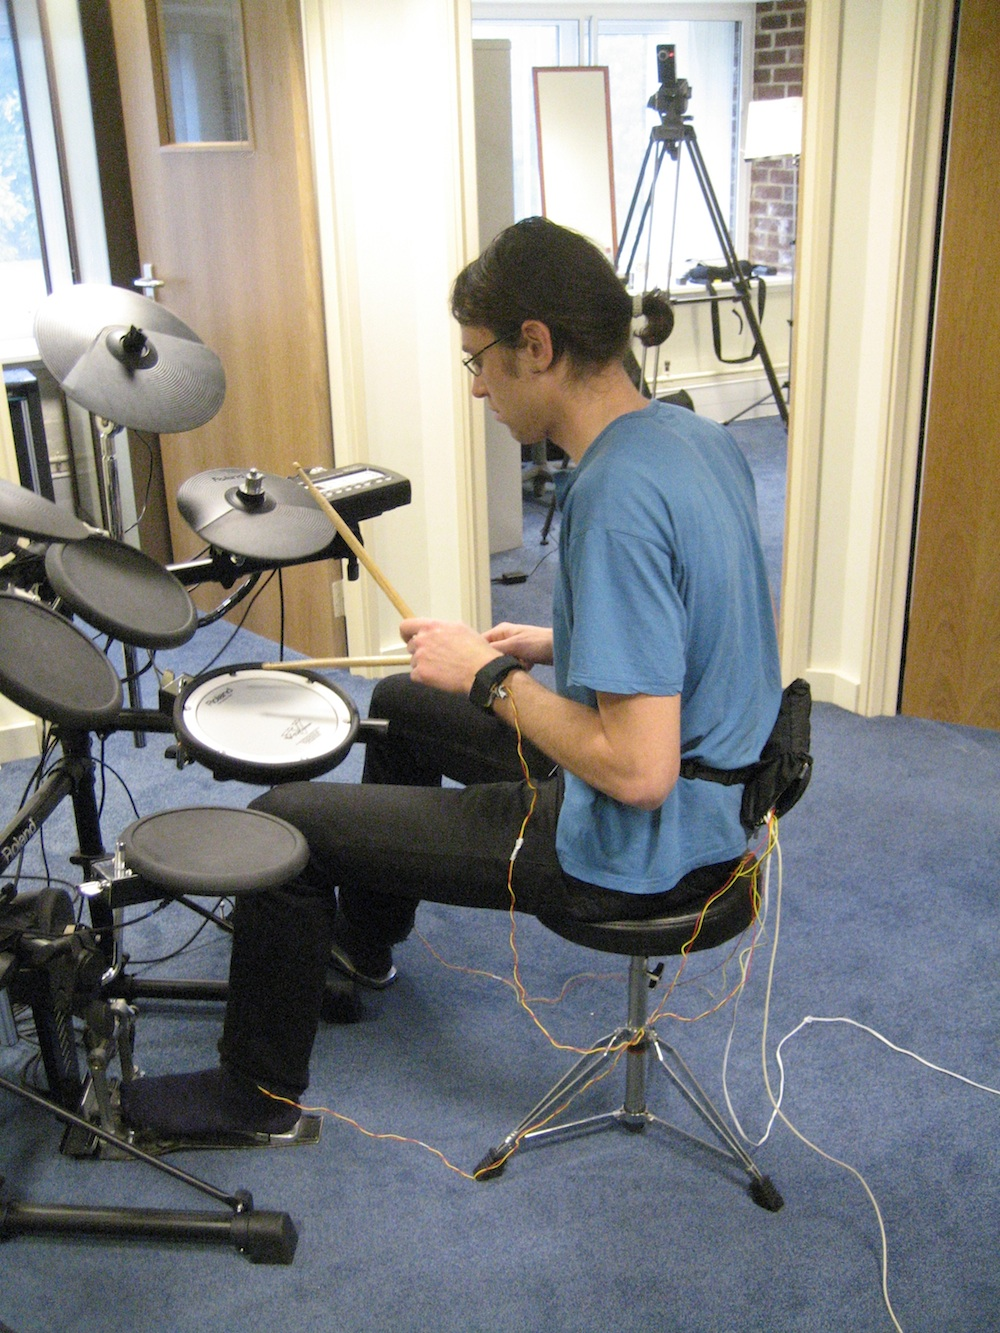
\includegraphics[width = \textwidth]{pictures/hapticdrumkit}
    \caption{Haptic Drum Kit \cite{10.1145/1709886.1709892}}
  \end{minipage}
  \hspace{0.1\textwidth}
  \begin{minipage}[b]{0.4\textwidth}
    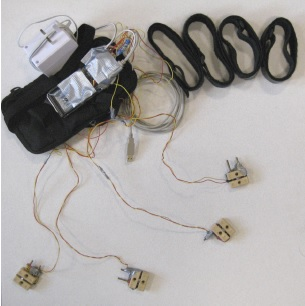
\includegraphics[width = \textwidth]{pictures/hapticdrumkit1}
    \caption{Vibratoren mit Bändchen und Tasche \cite{10.1145/1709886.1709892}}
  \end{minipage}
\end{figure}

\subsection{Haptic Guidance System}
Graham Grindlay \cite{4479984} vergleicht in seiner Arbeit wie gut sich ein einfacher Rhythmus mit haptischer Führung im Vergleich zu auditiven Lernen, erlernen lässt.
Dabei beschreibt er die Ähnlichkeit seiner Konstruktion zu dem Führen der Hand des Schülers durch den Lehrer.
Zu dieser Methode greifen viele Lehrer, weil das verbale Beschreiben nicht ausreicht, um eine komplizierte Bewegung genau zu erklären.
Allerdings entspricht das Führen nicht unbedingt der exakt richtigen Bewegung und ist eingeschränkt, was Geschwindigkeit und Stärke angeht.
Graham Grindlay will mit seinem Haptic Guidance System die Bewegungsgenauigkeit und -geschwindigkeit verbessern und das Lernen erleichtern.

\subsubsection{Aufbau}
Das Haptic Guidance System ist auf einen Freiheitsgrad eingeschränkt und fokussiert sich nur auf die Bewegung des Handgelenks.
Somit können nur einhändige Rhythmen trainiert werden.
Trotzdem gibt es viele rhythmische Aufgaben, die gerade für Anfänger wichtig sind.
Das Gerät hat nicht nur die Möglichkeit die Hand zu leiten, sondern kann auch vom Rotor getrennt werden, um einen Bewegung ohne Schwierigkeiten aufzunehmen.
Aufgenommene Bewegung können umgekehrt auch wieder abgespielt werden.
Auf diese Art wurden die Rhythmen für das audiobasierte Lernen aufgenommen, damit der Ton einen möglichst geringen Unterschied zum Gespielten auweist.
Damit alle Probanden eine gleiche Armhaltung einnehmen, ist das Haptic Guidance System mit einer Unterarmschale und einem Gurt versehen.
Als Sicherheitsmaßnahmen sind ein Knopf zum stoppen und Einschränkungsstangen installiert, damit das Handgelenk nicht unnatürlich bewegt werden kann.
Die Probanden haben verschiedene Rhythmen auditiv, dann haptisch und am Ende auditiv und haptisch gelernt.


\subsubsection{Ergebnisse}
Die Aufnahmen wurden in zeitlicher Präzision und Aufschlaggeschwindigkeit verglichen und es hat sich gezegt, dass das Hören wichtig ist für die zeitliche Präzision.
Die haptische Führung das Lernen der Aufschlaggeschwindigkeit erleichtert hat.
Da die Studie nur aus Kurzzeitmessungen bestand, lässt sich sagen, dass eine Kombination von auditiven und haptischen Lernen gerade am Anfang von Vorteil ist, um die richtige Bewegung mit der richtigen Geschwindigkeit und zeitlicher Präzision zu vereinen.


\begin{figure}
  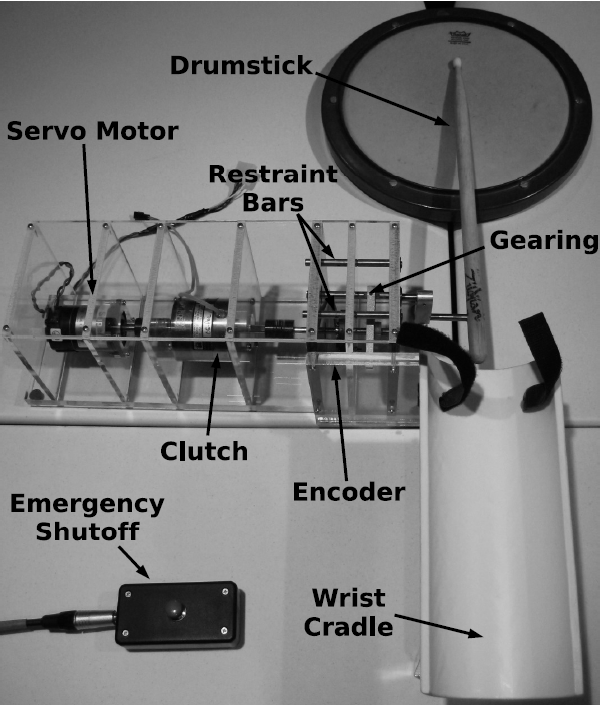
\includegraphics[width = 0.5\textwidth]{pictures/hapticdrumstick1}
  \caption{The Haptic Guidance System Hardware \cite{4479984}}
\end{figure}

\subsection{vibrotactile vest and ankle bands}
In Lee und Seungmoon Choi \cite{6775447} verwenden eine Weste mit Vibrationsgeräten und Bänder an den Knöcheln mit Vibratoren um ein komplettes Schlagzeug anzusteuern.

\begin{figure}
  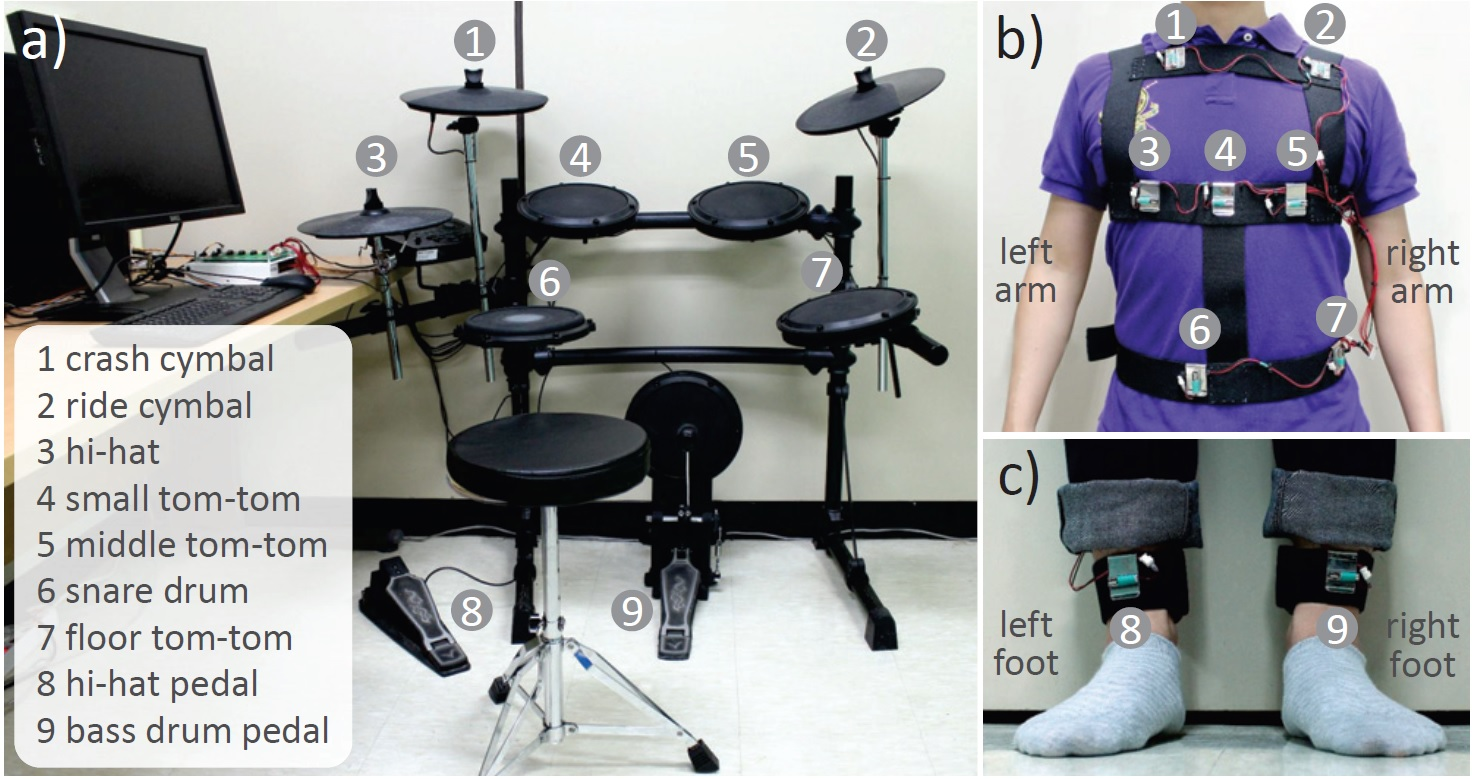
\includegraphics[width = \textwidth]{pictures/vibrotactilevest2}
  \caption{Vibrotaktile Weste mit Knöchelbändern und Midi-Drum Kit\cite{6775447}}
\end{figure}

\section{Passives Lernen durch Haptische Wearables}

\subsection{Haptic iPod}
Die Arbeit von Bouwer, Dalgleish und Holland\cite{bouwer2011haptic} basiert auf den Ergebnissen zum Haptic Drum Kit \cite{10.1145/1709886.1709892} und beschäftigt sich mit der Frage, ob sich mehrgliedrige Rhythmen auch passiv lernen lassen.
Dabei werden lautlos rhythmische Reize über die Haptischen Sensoren abgespielt, während sich die Probanden mit anderen Aufgaben beschäftigen.
Das verwendete System wird Haptic iPod genannt.
\subsubsection{Aufbau}
Der Haptic iPod existiert in zwei verschiedenen Versionen.
Eine portable Feldversion mit im Vorhinein aufgenommenen vierspurigen Stücken und batteriebetriebenen Kopfhörerverstärkern.
Dazu noch eine statische Testversion die mit einem Laptop bedient wird und mit stärkeren Kopfhörerverstärkern ausgestattet ist.
Für die Studie wurde die statische Testversion verwendet.
Die Probanden spielten zu Anfang möglichst schwere Rhythmen nach Gehör.
Danach wurden 2 Rhythmen aus den gespielten Rhythmen ausgewählt und abwechselnd über die haptischen Wearables abgespielt, während eine 30 minütige Leseverständnis Aufgabe bearbeitet wurde.
Im Anschluss sollten die Rhythmen vom Anfang wiederholt werden.
Die Ergebnisse wurden auf Genauigkeit, Timing, Anzahl der Versuche und Fehleranzahl im besten Versuch verglichen.
Zum Schluss wurden die Probanden zu ihren Erfahrungen und Einstellungen zum Haptic iPod befragt.

\subsubsection{Ergebnisse}
Wie auch beim Haptic Drum Kit \cite{10.1145/1709886.1709892} ist die Haptik gegenüber dem Gehör im Vorteil, wenn es darum geht, welche Gliedmaßen zu verwenden ist.
Es wurde sich auch die Kombination aus Gehör und Haptik gewünscht, wie auch Portabilität und Kabellosigkeit.
Die Haptik hat keinen Vorteil, wenn es darum geht, welche Trommel zu spielen ist und die Wearables sind über die Zeit unangenehm zu tragen gewesen.
Das passive Lernen macht es auch schwerer sich auf eine Aufgabe zu konzentrieren und fordert das setzen von Prioritäten.

\section{The Haptic Bracelets}
Haptisches Lernen kann mit gleichem Erfolg genutzt werden, wie auditives Lernen um Rhythmen zu erlernen, die Mehrgliedrige Koordination benötigen.
Die Kombination von beidem ist den einzelnen Lernmethoden vorzuziehen.
Haptisches Lernen hat Vorteile, wenn es darum geht, welche Gliedmaßen für welche Aktionen benötigt werden.
Bietet allerdings auch Nachteile, da starke körperliche Bewegung das haptische Signal überdecken kann. \cite{bouwer2013haptic}

\section{Zusammenfassung}
\subsection{Ergebnisse}
Haptisches Lernen kann das herkömmliche Lernen mit Gehör und Lehrer bis jetzt nicht ersetzen, bietet aber eine interessante zusätzliche Lernmöglichkeit.
Es bietet Abwechslung und die Möglichkeit des passiven Lernens.
Zudem ist eine Kombination von auditiven und haptischen Lernen erfolgreicher und spannender für den Schüler.

\subsection{Ausblick}
In der Zukunft können Haptische Wearables in Gesundheit, Unterhaltung, Sicherheit und vielen weiteren Gebieten, die noch nicht identifiziert und untersucht wurden, eingesetzt werden.
Derzeitige Vibrationsgeräte in Smartphones könnten durch verschiedene Rhythmen mehr Informationenen übertragen.
Außerdem können haptische Wearables Verwendung in weiteren physisch komplexen Fähigkeiten wie Tanzen, Sport oder Medizin finden. %( remote medicine)


\bibliographystyle{splncs03}
\bibliography{proseminar}
\end{document}
